%%%%%%%%%%%%%%%%%%%%%%%%%%%%%%%%%%%%%%%%%%%%%%%%%%%%%%%%%%%%%%%%%%%%
%% I, the copyright holder of this work, release this work into the
%% public domain. This applies worldwide. In some countries this may
%% not be legally possible; if so: I grant anyone the right to use
%% this work for any purpose, without any conditions, unless such
%% conditions are required by law.
%%%%%%%%%%%%%%%%%%%%%%%%%%%%%%%%%%%%%%%%%%%%%%%%%%%%%%%%%%%%%%%%%%%%

% This theme was based on fibeamer theme 
% If you found any bugs please contact @karlosos
% This repository is hosted on github https://github.com/karlosos/zut-fibeamer/

\documentclass{beamer}
\usetheme[faculty=wi]{fibeamer}
\usepackage[utf8]{inputenc}
\usepackage[
  main=polish,
  polish
]{babel}

\usepackage{color}
\definecolor{lightgray}{rgb}{0.95, 0.95, 0.95}
\definecolor{darkgray}{rgb}{0.4, 0.4, 0.4}
%\definecolor{purple}{rgb}{0.65, 0.12, 0.82}
\definecolor{editorGray}{rgb}{0.95, 0.95, 0.95}
\definecolor{editorOcher}{rgb}{1, 0.5, 0} % #FF7F00 -> rgb(239, 169, 0)
\definecolor{editorGreen}{rgb}{0, 0.5, 0} % #007C00 -> rgb(0, 124, 0)
\definecolor{orange}{rgb}{1,0.45,0.13}		
\definecolor{olive}{rgb}{0.17,0.59,0.20}
\definecolor{brown}{rgb}{0.69,0.31,0.31}
\definecolor{purple}{rgb}{0.38,0.18,0.81}
\definecolor{lightblue}{rgb}{0.1,0.57,0.7}
\definecolor{lightred}{rgb}{1,0.4,0.5}
\usepackage{upquote}
\usepackage{listings}

% CSS
\lstdefinelanguage{CSS}{
  keywords={color,background-image:,margin,padding,font,weight,display,position,top,left,right,bottom,list,style,border,size,white,space,min,width, transition:, transform:, transition-property, transition-duration, transition-timing-function},	
  sensitive=true,
  morecomment=[l]{//},
  morecomment=[s]{/*}{*/},
  morestring=[b]',
  morestring=[b]",
  alsoletter={:},
  alsodigit={-}
}

% JavaScript
\lstdefinelanguage{JavaScript}{
  morekeywords={typeof, new, true, false, catch, function, return, null, catch, switch, var, if, in, while, do, else, case, break},
  morecomment=[s]{/*}{*/},
  morecomment=[l]//,
  morestring=[b]",
  morestring=[b]'
}

\lstdefinelanguage{HTML5}{
  language=html,
  sensitive=true,	
  alsoletter={<>=-},	
  morecomment=[s]{<!-}{-->},
  tag=[s],
  otherkeywords={
  % General
  >,
  % Standard tags
	<!DOCTYPE,
  </html, <html, <head, <title, </title, <style, </style, <link, </head, <meta, />,
	% body
	</body, <body,
	% Divs
	</div, <div, </div>, 
	% Paragraphs
	</p, <p, </p>,
	% scripts
	</script, <script,
  % More tags...
  <canvas, /canvas>, <svg, <rect, <animateTransform, </rect>, </svg>, <video, <source, <iframe, </iframe>, </video>, <image, </image>, <header, </header, <article, </article
  },
  ndkeywords={
  % General
  =,
  % HTML attributes
  charset=, src=, id=, width=, height=, style=, type=, rel=, href=,
  % SVG attributes
  fill=, attributeName=, begin=, dur=, from=, to=, poster=, controls=, x=, y=, repeatCount=, xlink:href=,
  % properties
  margin:, padding:, background-image:, border:, top:, left:, position:, width:, height:, margin-top:, margin-bottom:, font-size:, line-height:,
	% CSS3 properties
  transform:, -moz-transform:, -webkit-transform:,
  animation:, -webkit-animation:,
  transition:,  transition-duration:, transition-property:, transition-timing-function:,
  }
}

\lstdefinestyle{htmlcssjs} {%
  % General design
%  backgroundcolor=\color{editorGray},
  basicstyle={\footnotesize\ttfamily},   
  frame=b,
  % line-numbers
  xleftmargin={0.75cm},
  numbers=left,
  stepnumber=1,
  firstnumber=1,
  numberfirstline=true,	
  % Code design
  identifierstyle=\color{black},
  keywordstyle=\color{blue}\bfseries,
  ndkeywordstyle=\color{editorGreen}\bfseries,
  stringstyle=\color{editorOcher}\ttfamily,
  commentstyle=\color{brown}\ttfamily,
  % Code
  language=HTML5,
  alsolanguage=JavaScript,
  alsodigit={.:;},	
  tabsize=2,
  showtabs=false,
  showspaces=false,
  showstringspaces=false,
  extendedchars=true,
  breaklines=true,
  % German umlauts
  literate=%
  {Ö}{{\"O}}1
  {Ä}{{\"A}}1
  {Ü}{{\"U}}1
  {ß}{{\ss}}1
  {ü}{{\"u}}1
  {ä}{{\"a}}1
  {ö}{{\"o}}1
}

\title{Tópicos especiais em Sistemas}
\subtitle{Javascript - NodeJS}
\author{Prof. Juliana Costa Silva}

\usepackage{ragged2e}  % `\justifying` text
\usepackage{booktabs}  % Tables
\usepackage{tabularx}
\usepackage{tikz}      % Diagrams
\usetikzlibrary{calc, shapes, backgrounds}
\usepackage{amsmath, amssymb}
\usepackage{url}       % `\url`s
\usepackage{listings}  % Code listings
\frenchspacing
\begin{document}

%------------------------------------------------------------------------
  \frame[c]{\maketitle}
  %\AtBeginSection[]{% Print an outline at the beginning of sections
    \begin{frame}<beamer>
      \frametitle{O que veremos hoje}
      \tableofcontents
    \end{frame}
%------------------------------------------------------------------------
    \section{Servidor JS}
    \begin{frame}{Node}
      \framesubtitle{Interpretador JS}%
      
      \begin{itemize}
            \item Se queremos associar a linguagem JavaScript ao browser, apesar de ser o formato em que ela é mais utilizada. Uma das ferramentas que usaremos para interpretar a linguagem e desenvolver nosso programa será o \textbf{NodeJs}.
            \item Acesse o terminal (cmd) e digite:  \textcolor{red}{node -v} (\textcolor{gray}{\textit{Você verá a versão do NodeJS instalada}}).
            \item Ainda no terminal (cmd) digite:  \textcolor{red}{node + ENTER}, (\textcolor{gray}{\textit{Você está no ambiente NodeJS que aguarada por comandos JS.}})
       \end{itemize}
       \tiny{Fonte: \cite{nodejs2022api}}
     \end{frame}
%------------------------------------------------------------------------
\section{Usando Arquivos}
\begin{frame}{Executar arquivos JS}

    \begin{itemize}
        \item Crie um arquivo chamado arquivo.js;
        \item Adicione o código \textcolor{blue}{console.log("Arquivo executado!!")};
        \item Acesse o terminal (cmd) via VSCode:  
    \end{itemize}
    \centering
	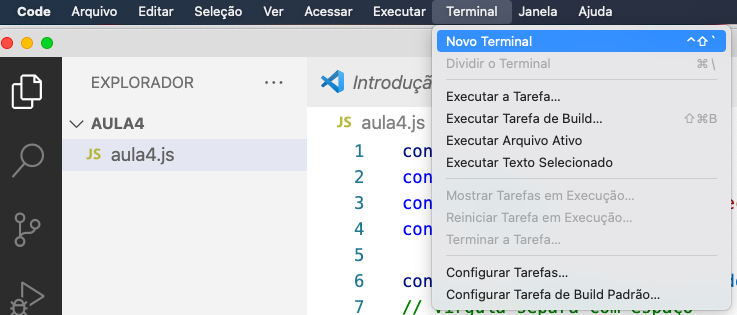
\includegraphics[width=80mm]{resources/aula_js_4_1.png}\\
            \tiny{ Acessando o terminal via VS Code \textbf{Fonte:} A autora.}
\end{frame}

%------------------------------------------------------------------------
\begin{frame}{Executar arquivos JS [2]}

    \begin{itemize}
        \item Ao acessar o terminal via VS Code, você não precisará navegar até o local do projeto, já estará nele.
        \item Digite \textcolor{red}{node arquivo.js}
        \item \textcolor{gray}{\textit{Você executou todo o arquivo js criado.}}
    \end{itemize}
    \centering
	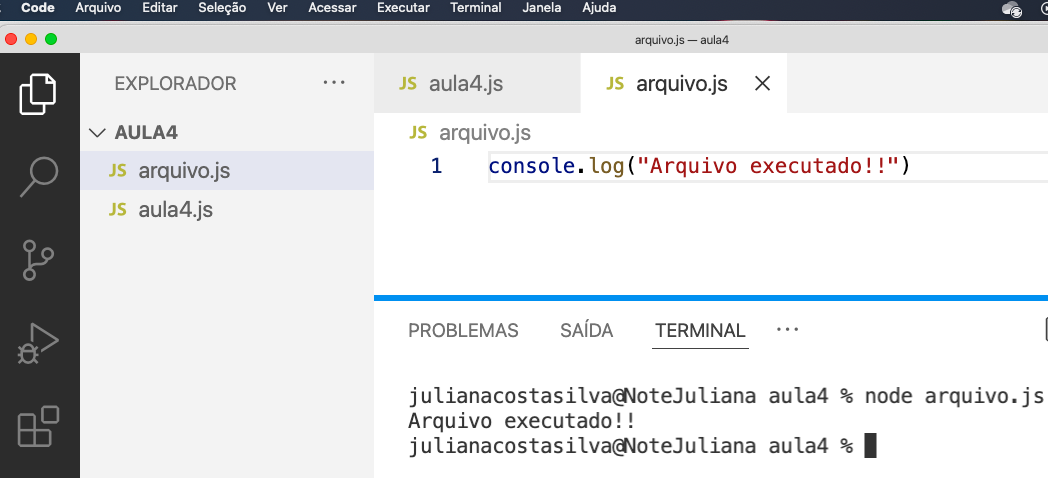
\includegraphics[width=80mm]{aulas/resources/aula_js_4_2.png}\\
            \tiny{ Executar arquivo js via terminal com VS Code \textbf{Fonte:} A autora.}
\end{frame}
%------------------------------------------------
\section{Tipos de variáveis}
\begin{frame}{Variáveis JS}
Teste o código abaixo:
    \centering
	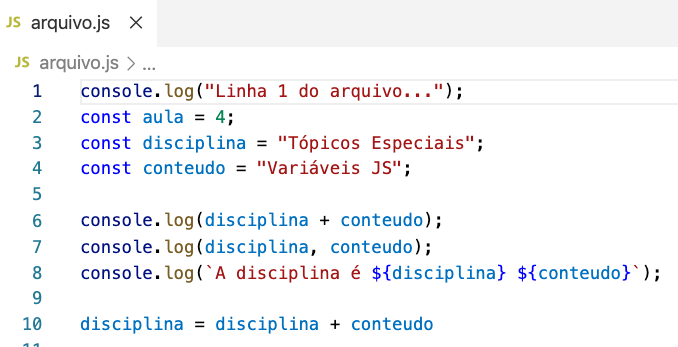
\includegraphics[width=80mm]{resources/aula_js_4_3.png}\\
    \tiny{ \textbf{Fonte:} A autora.}\\
    Execute arquivo.js via terminal pelo VS Code.
\end{frame}
%-----------------------------------------------------
    \begin{frame}{Resultado}
    \centering
	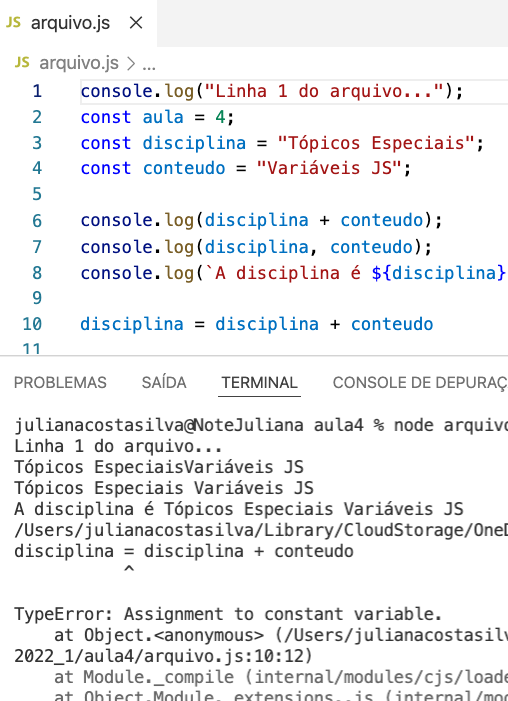
\includegraphics[width=50mm]{resources/aula_js_4_4.png}\\
            \tiny{\textbf{Fonte:} A autora}\\
            \textcolor{purple}{TypeError: Assignment to constant variable.}
    \end{frame}
%-----------------------------------------------------
    \begin{frame}{Declaração de variáveis JS}
    \begin{block}{O que é uma variável?}
    Uma variável é um container para um valor, como um número que podemos usar em uma operação de adição, ou uma sequência de texto que possamos usar como parte de uma oração. Mas uma coisa especial a respeito das variáveis é que seu conteúdo pode mudar.
    \end{block}
    \centering
    \vspace{0.5cm}
    \tiny{\textbf{Fonte:} \cite{moziladev2022js}}
    \end{frame}
    
%-----------------------------------------------------
    \begin{frame}{A diferença entre \textcolor{blue}{var} e \textcolor{blue}{let}}
    \begin{block}{var}
    Quando o JavaScript foi criado, havia apenas \textcolor{yellow}{var}. Isso funciona basicamente bem na maioria dos casos, mas tem alguns problemas na maneira como funciona, seu design pode ser confuso ou totalmente irritante.
    \end{block}
    
    \begin{block}{let}
    A declaração \textcolor{yellow}{let} foi criada nas versões modernas de JavaScript, uma nova palavra-chave para criar variáveis que funcionam de maneira um pouco diferente de \textcolor{yellow}{var}, corrigindo seus problemas no processo.
    \end{block}
    \centering
    %\vspace{0.5cm}
    \tiny{\textbf{Fonte:} \cite{moziladev2022js}}
    \end{frame}
    
%-----------------------------------------------------
\begin{frame}{A diferença entre \textcolor{blue}{var} e \textcolor{blue}{let} [2]}
    \begin{block}{var}
    \begin{itemize}
        \item A declaração \textcolor{yellow}{var} permite declarar uma variável depois que você a inicializa, isso resulta em código confuso e difícil de entender.
        \item Ao usar \textcolor{yellow}{var}, você pode declarar a mesma variável quantas vezes quiser. 
    \end{itemize}
    \end{block}
    
    \begin{block}{let}
    \begin{itemize}
        \item Com \textcolor{yellow}{let} você não consegue declarar uma variável depois que você a inicializa. 
        \item Com \textcolor{yellow}{let} você não consegue declarar uma variável varias vezes. 
        \item Com \textcolor{yellow}{let} é possível apenas atualizar o valor de uma variável, não declara-lá novamente.
    \end{itemize}
    \end{block}
    \centering
    %\vspace{0.5cm}
    \tiny{\textbf{Fonte:} \cite{moziladev2022js}}
\end{frame}
    %TIPOS: 
    %Arrays - https://developer.mozilla.org/pt-BR/docs/Learn/JavaScript/First_steps/Variables
%-----------------------------------------------------
\section{Atividade} 
\begin{frame}{Atividade}
	Com base no conteúdo da aula de hoje DESENVOLVA:
	\begin{enumerate}
	    \item  Uma página web que exiba um texto para cada seleção em uma select;
	    \item As opções devem ser sobre JavaScript:
	    \item Opção let: deve explicar o que let faz;
	    \item Opção var: deve explicar o que var faz;
	    \item Opção const: deve explicar o que const faz;
	\end{enumerate}
\end{frame}
%--------------------------------------------------------
\section{NodeJS}
\begin{frame}{NodeJS}
    \begin{block}{O que é?}
        Um \alert{JS Runtime Enviroment}: Ambiente de execução Javascript.
  \end{block}
  \begin{exampleblock}{O que ele não é?}        
    Não é um framework, nem uma linguagem de programação.
  \end{exampleblock}
  \begin{alertblock}{Pra que serve??}
    Para desenvolvimento de aplicações Javascript, backend, frontend, APIs, microserviços.
  \end{alertblock}
\end{frame}
%--------------------------------------------------------
\begin{frame}{Vantagens NodeJS}
	\begin{itemize}
	\item Rápido;
	\item Alta escalabilidade
	\item Ecosistema muito grande (NPM)
	\item Empresas como: Netflix e PayPal utilizam.
	\item Javascript (front, back mobile... tudo)
	\end{itemize}
\end{frame}
%-------------------------------------------------
\begin{frame}{Funcionamento NodeJS}
    
\includegraphics[width=90mm]{resources/aula1_5.png}\\
    \tiny{\textbf{Fonte:} \cite{ich2021}}
\end{frame}
%----------------------------------------------------
    \begin{frame}{Funcionamento NodeJS}
      \begin{columns}[onlytextwidth]
        \column{.5\textwidth}
          \alert{Node.js} é escrito não apenas em Javascript, mas também em $C++$ e Javascript. \\
          Para operar corretamente, depende de muitas bibliotecas. \\
          No entanto, V8 e LIBUV são duas dependências mais importantes que tratam da maioria das operações do Node.js.

        \column{.5\textwidth}
            
\includegraphics[width=55mm]{resources/aula1_6.png}\\
            \tiny{\textbf{Fonte:} \cite{ich2021}}

      \end{columns}
    \end{frame}
    
 %-------------------------------------------------------
    \begin{frame}{Funcionamento V8]}
      \begin{columns}[onlytextwidth]
        \column{.5\textwidth}
          Node.js é construído no motor V8 do Google. Este é um mecanismo de javascript rápido. \\
          O motor V8 tem o papel de converter o código javascript em código de máquina que o computador entende.\\
          \vspace{0.5cm}
	O Node.js não entende o código javascript que escrevemos sem o V8.
        \column{.5\textwidth}
            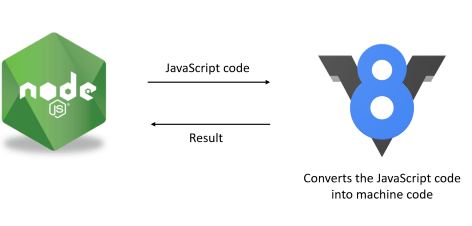
\includegraphics[width=65mm]{resources/aula1_7.png}\\
            \tiny{\textbf{Fonte:} \cite{ich2021}}
      \end{columns}
    \end{frame}
    
%------------------------------------------------------
\begin{frame}{Entrada e saída Assíncrona}
    \framesubtitle{O que é isso?}%
    LIBUV é outra  dependência do Node.js. Esta dependência permite ao Node o acesso ao sistema operacional da máquina, rede, sistema de arquivos e muito mais.\\
          \vspace{0.5cm}
    LIBUV é uma biblioteca de código aberto com um forte foco em E / S assíncrona (entrada-saída). LIBUV é escrito em C ++. Além de focar na E / S assíncrona, LIBUV também implementa dois recursos importantes que são o loop de eventos e o pool de threads.          
\end{frame}
%-------------------------------------------------------
\begin{frame}{Loops e Eventos}
    \framesubtitle{O que é isso?}%
    \begin{columns}[onlytextwidth]
    \column{.5\textwidth}
    Quando usamos Node.js em um computador, significa que há um processo de nó em execução nesse computador. 
         \\
	Nesse processo, o Node.js é executado em uma única thread. \\
	O que é importante entender aqui, é o fato de que o nó roda em apenas um thread, por exemplo, se tivermos 4 tarefas diferentes, então todas essas quatro tarefas acontecerão em uma única thread.          
    \vspace{0.5cm}
    \column{.5\textwidth}
        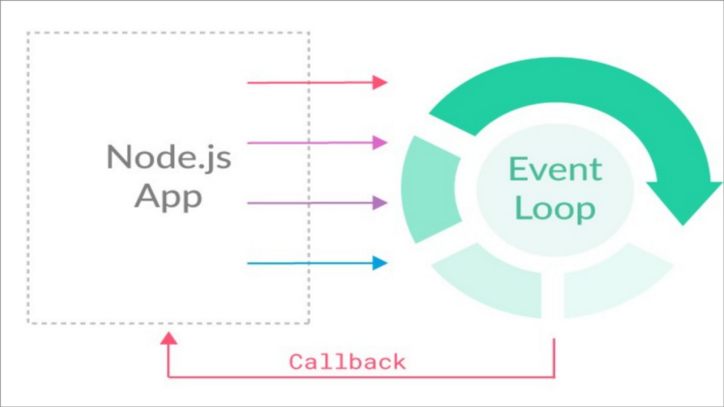
\includegraphics[width=65mm]{resources/aula1_8.png}\\
        \tiny{\textbf{Fonte:} \cite{ich2021}}
    \end{columns}
\end{frame}
%------------------------------------------------------------------------
    \section{Introdução}
    \begin{frame}{O que precisaremos?}
      \framesubtitle{Instalações necessárias}%
      
      \begin{itemize}
            \item Instalação da verão "LTS" do NodeJs
            \item Esta é a última versão estável e suporte do Node.
            \item VSCode
       \end{itemize}
     \end{frame}
%------------------------------------------------------------------------
%    \begin{frame}[label=lists]{Ferramentas e tecnologias}
%      \begin{columns}[onlytextwidth]
%        \column{.5\textwidth}
%          \begin{itemize}
%            \item NodeJS \textcolor{gray}{(instalar até a próxima aula)}
%            \item VSCode \textcolor{gray}{(ou outra IDE da preferência do aluno)}
%            \item AngularJS 
%          \end{itemize}
%        \column{.5\textwidth}
%            
\includegraphics[width=55mm]{resources/aula1_4.png}
%      \end{columns}
%    \end{frame}

%------------------------------------------------------------------------
    \subsection{Criando um projeto NodeJS}
    \begin{frame}[label=simmonshall]{Versão NodeJS}

      \begin{block}{Teste a Instalação}
        Uma vez que instalação estiver concluída, abriremos o VSCode e por meio do terminal verificaremos que o Node fato foi instalado e sua versão. \\
        Escreveremos o comando \alert{node -v} para acessarmos essa informação.\\
        No caso do nosso projeto, a versão utilizada e v14.16.0.
      \end{block}
      \begin{exampleblock}{NPM}
        Para iniciarmos nosso projeto em Node, vamos usar um gerenciador de módulos.\\
        Para isto usaremos o NPM, ou \textit{Node Package Manager}.\\
        O Node já instala o NPM automaticamente.\\
        Verifique no terminal pelo comando \alert{npm -v}, sua versão.
      \end{exampleblock}
    \end{frame}
%------------------------------------------------------------------------
    \begin{frame}[label=proof]{Iniciando o projeto}
	\begin{itemize}
	\item Navegue até a pasta onde deseja criar o projeto;
	\item Use o comando \alert{npm init} dentro da pasta onde deseja criar seu projeto;
	\end{itemize}
	Continua...
    \end{frame}
    
       %------------------------------------------------------------------------
    \begin{frame}[label=lists]{Iniciando um projeto}
    \begin{exampleblock}{Perguntas...}
        	\begin{itemize}
	\item package name (nome do projeto);
	\item version; 
	\item description; 
	\item entry point ( \textit{arquivo que irá inicializar o servidor. Não temos ainda esse arquivo mas ele se chamará index.js quando criarmos o servidor}); 
	\item test command; 
	\item git repository; 
	\item keywords; 
	\item autor (nosso nome); 
	\item license (\textit{licença ISC}).
        	\end{itemize}
      \end{exampleblock}
            %
\includegraphics[width=90mm]{resources/aula1_5.png}\\
            %\tiny{\textbf{Fonte:} \cite{ich2021}}
    \end{frame}
    %------------------------------------------------------------------------
    \begin{frame}[label=lists]{package.json}
          Confirmando as informações e um arquivo chamado \textbf{package.json} terá sido criado. \\
          Este arquivo contem todas as informações do nosso projeto, desde o nome, sua versão e scripts que podem ser executados até novos pacotes que poderemos instalar.

    \end{frame}
    
 %------------------------------------------------------------------------
 \subsection{Editando seu projeto}
    \begin{frame}{Trabalhando no projeto}
      \begin{columns}[onlytextwidth]
        \column{.5\textwidth}
         Vamos criar nosso arquivo \textit{entry point}, este arquivo será o principal do projeto, responsável pela execução do servidor;\\
        
          \vspace{0.5cm}
	Crie o arquivo com o nome \textbf{index.js}.
        \column{.5\textwidth}
            \pause
            \begin{itemize}
		\item Vamos utilizar o Express;
		\item Express é um módulo do Node que contém uma biblioteca que possibilitará essa execução com o servidor;
		\item Para instala digite no terminal \alert{ npm install express}
	\end{itemize}
      \end{columns}
      Observe as dependências criadas no arquivo \textbf{package.json}.
    \end{frame}
    
  %------------------------------------------------------------------------
    \begin{frame}{Editando o index.js}
	No arquivo \textbf{index.js}, vamos declarar uma contante Js de nome express, que vai ser inicializada com o módulo express
	
          \vspace{0.5cm}
          Use o seguinte comando:\\
          \alert{const express = require('express') }          
          
    \end{frame}
    
 %------------------------------------------------------------------------
    \begin{frame}{Mais sobre Express}

      \begin{columns}[onlytextwidth]
        \column{.5\textwidth}
         Utilizamos uma string pois nos referimos a uma biblioteca.\\
         O express terá várias funções, e uma delas é o aplicativo que será executado no servidor. \\
         Inseriremos também a porta que o servidor deve escutar para acessar requisições. \\
         Essa porta será a 3000, e por enquanto inseriremos apenas um console.log() com uma mensagem de texto.        
          \vspace{0.5cm}
	
        \column{.5\textwidth}
            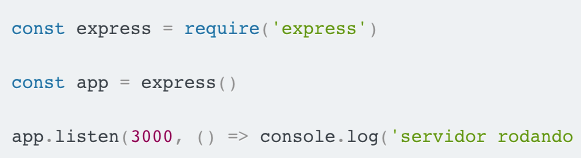
\includegraphics[width=65mm]{resources/aula2_1.png}\\
            \tiny{\textbf{Fonte:} O autor}

      \end{columns}
    \end{frame}
    %----------------------------------------------------------------
     \begin{frame}{Execute seu projeto}
    Para executarmos esse servidor, no console escreveremos o comando \alert{node index.js}. \\
    Veremos a mensagem 'servidor rodando na porta 3000', como esperávamos.
    \vspace{0.5cm}

	Se acessarmos no navegador o caminho \alert{localhost:3000} teremos algo em execução, mas não encontramos nenhum get, afinal não criamos nenhuma rota ainda.
    \end{frame}
%--------------------------------------------------------
\section{Referências}
    \begin{frame}{Referências}%[allowframebreaks]
\frametitle{Referências}
\small
\begin{center}
\tiny
\bibliographystyle{apalike}
\bibliography{ref_aula}
\end{center}
\end{frame}
%--------------------------------------------------------
\end{document}
